% !TEX root = msc_thesis.tex

- Statistics on homology modelling coverage

- Accuracy over different sequence identity bins

- within protein correlation on the test set


\clearpage

% === CORE ===

% Training set stats

\begin{figure}[h]
	\centering
	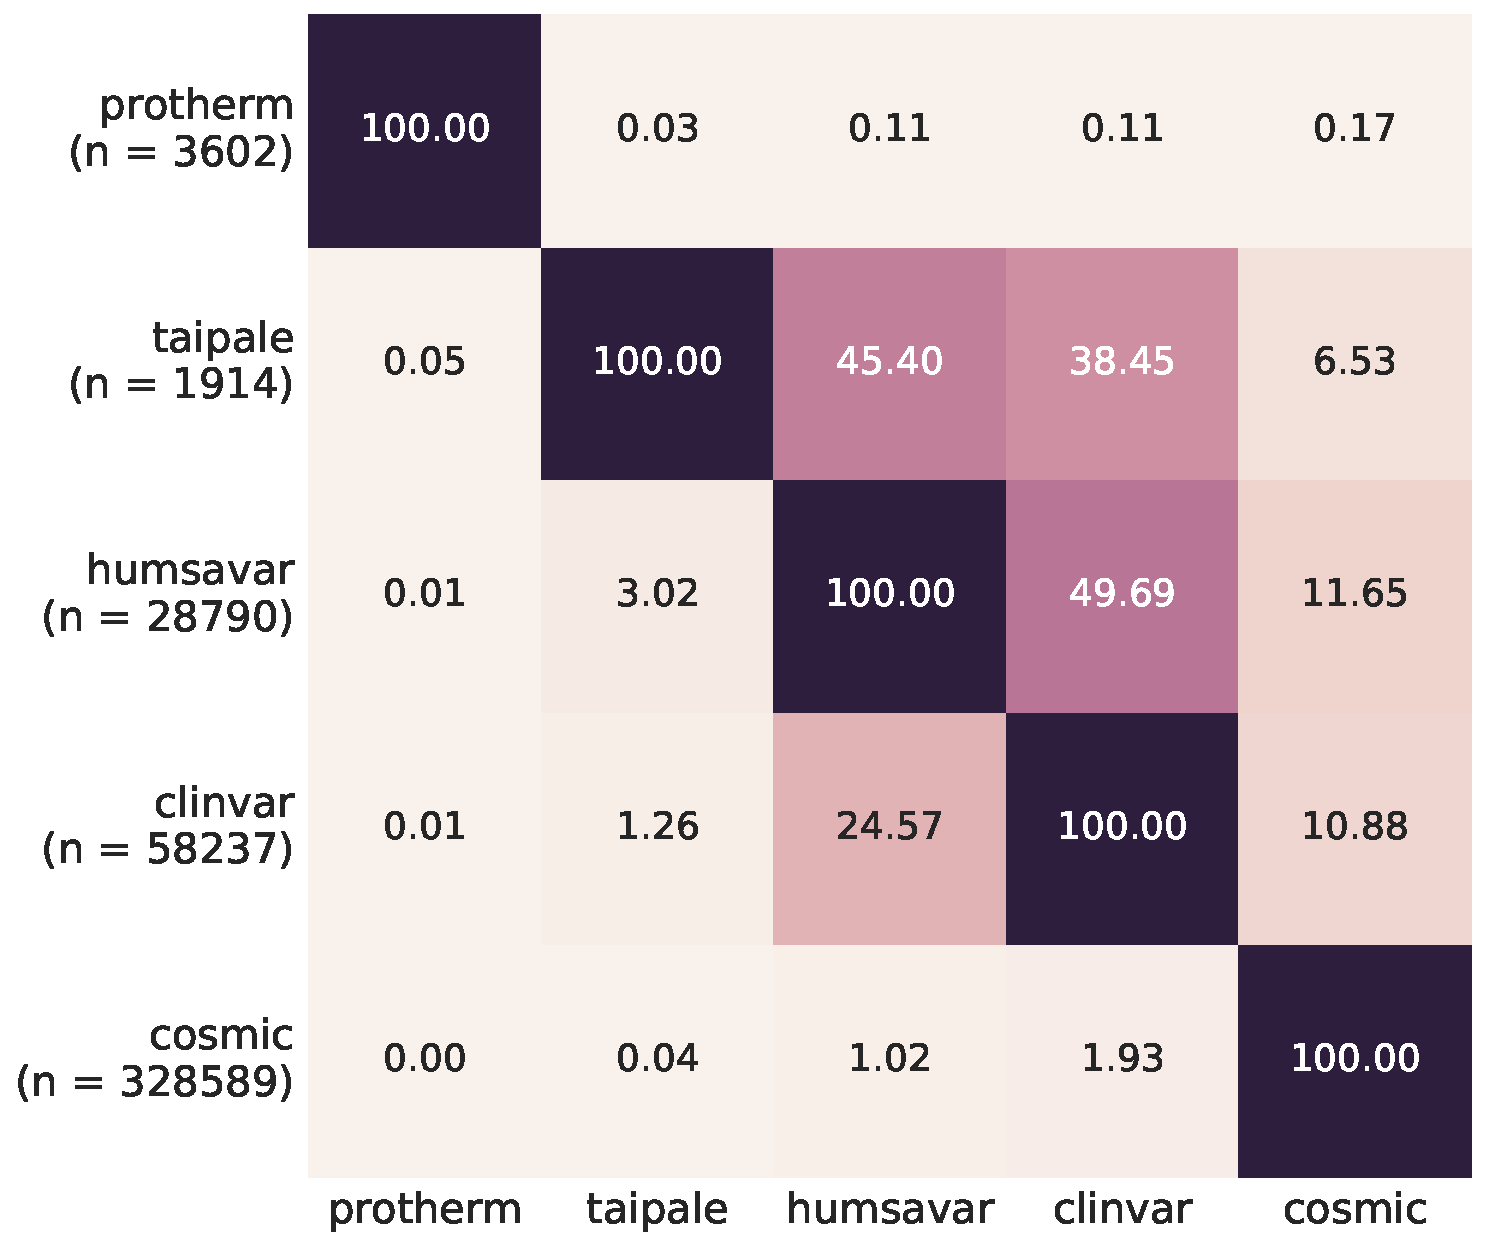
\includegraphics[width=0.65\textwidth]{static/elaspic_training_set/core_data_statistics/training_set_overlap_final.pdf}
	\caption{Size and overlap between the core and interface predictor datasets.}
\end{figure}


\begin{table}[h]
\caption{Description of the dataset used to train the core predictor.} \label{tab:core_datasets}
\begin{tabular}{l | p{13cm}}
	\toprule
	Dataset name & Experimental feature \\
	\midrule
	Protherm \cite{kumar_protherm_2006} & Change in the Gibbs free energy of protein folding ($\Delta \Delta G$). \\
	Taipale \cite{sahni_widespread_2015} & Change in the interaction with various quality control factors (QCFs), measured using the LUMIER assay. \\
	Humsavar \cite{consortium_uniprot:_2015} & $1$ if the mutation is annotated with at least one disease in the UniProt \textit{humsavar.txt} file. $0$ if the mutation is annotated as ``Polymorphism'' in the UniProt \textit{humsavar.txt} file. \\
	ClinVar \cite{landrum_clinvar:_2016} & $1$ if the mutation is found in the ClinVar \textit{clinvar\_20160531.vcf} file. $0$ if the mutation is found in the ClinVar \textit{common\_no\_known\_medical\_impact\_20160531.vcf} file. \\
	COSMIC \cite{forbes_cosmic:_2015} & $1$ if the mutation is predicted to be deleterious by FATHMM in the COSMIC database. $0$ if the mutation is predicted to be benign by FATHMM in the COSMIC database. \\
	\bottomrule
\end{tabular}
\end{table}

% Machine learning

\begin{figure}[h]
	% \centering
	\begin{subfigure}[b]{0.6\textwidth}
		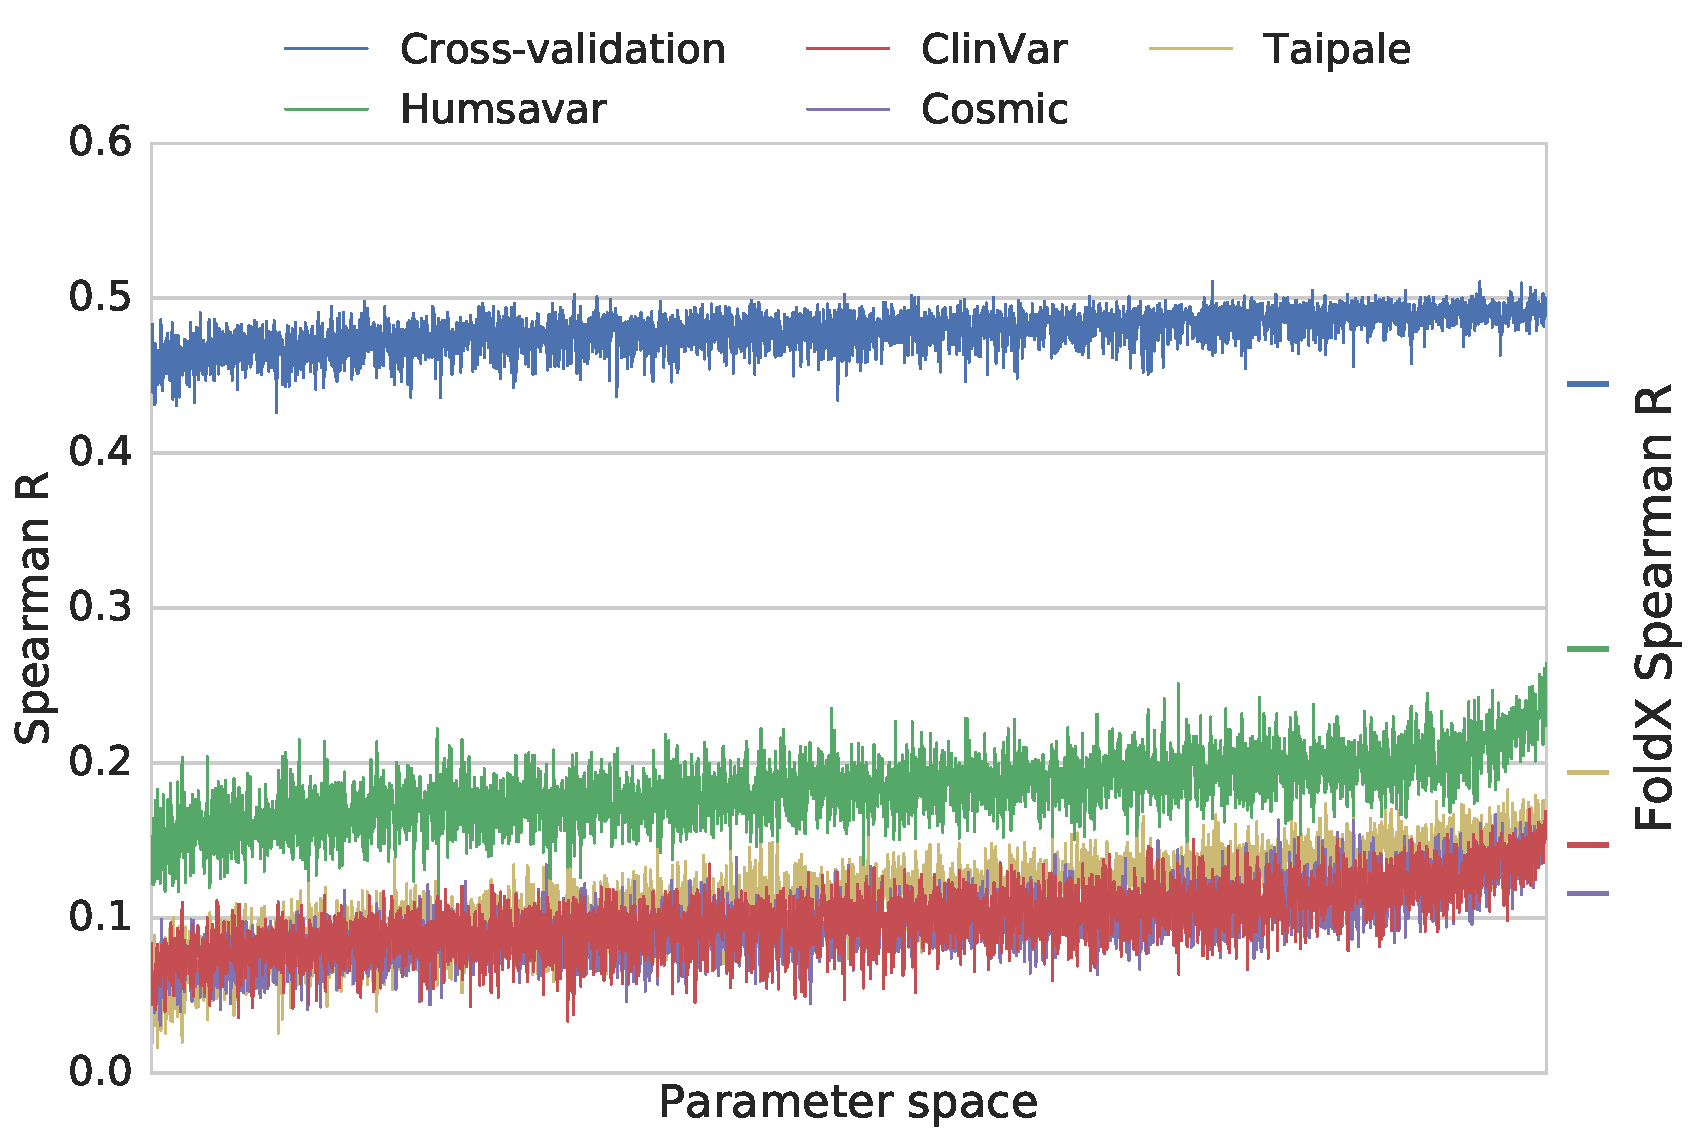
\includegraphics[width=1\linewidth]{static/elaspic_training_set/core_machine_learning/gridsearch.pdf}
		\caption{Grid-search over parameter space.}
		\label{fig:Ng1}
	\end{subfigure}

	\begin{subfigure}[b]{0.75\textwidth}
		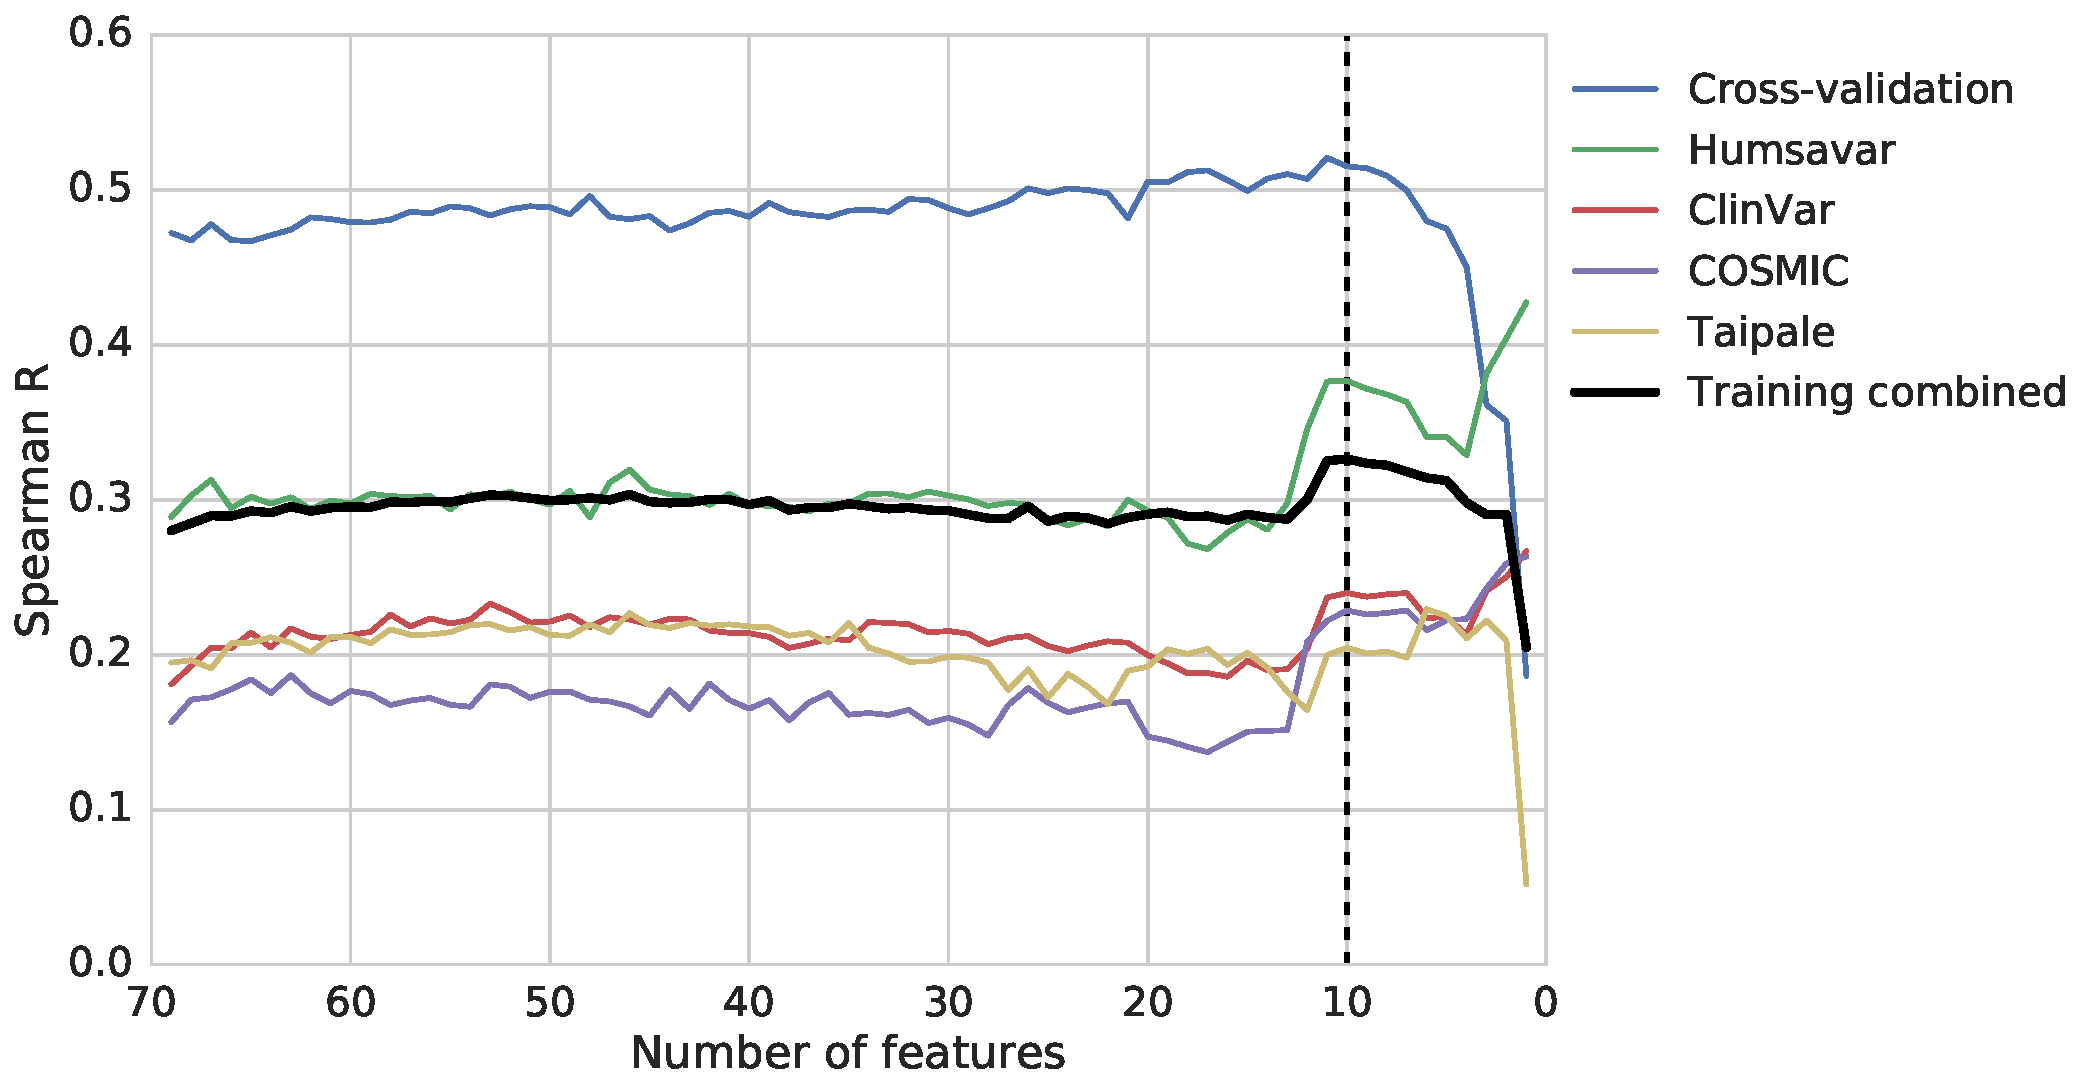
\includegraphics[width=1\linewidth]{static/elaspic_training_set/core_machine_learning/feature_elimination.pdf}
		\caption{Feature elimination.}
		\label{fig:Ng1}
	\end{subfigure}

	\caption{Machine learning pipeline.}
\end{figure}


\clearpage

\begin{figure}[h]
	\centering
	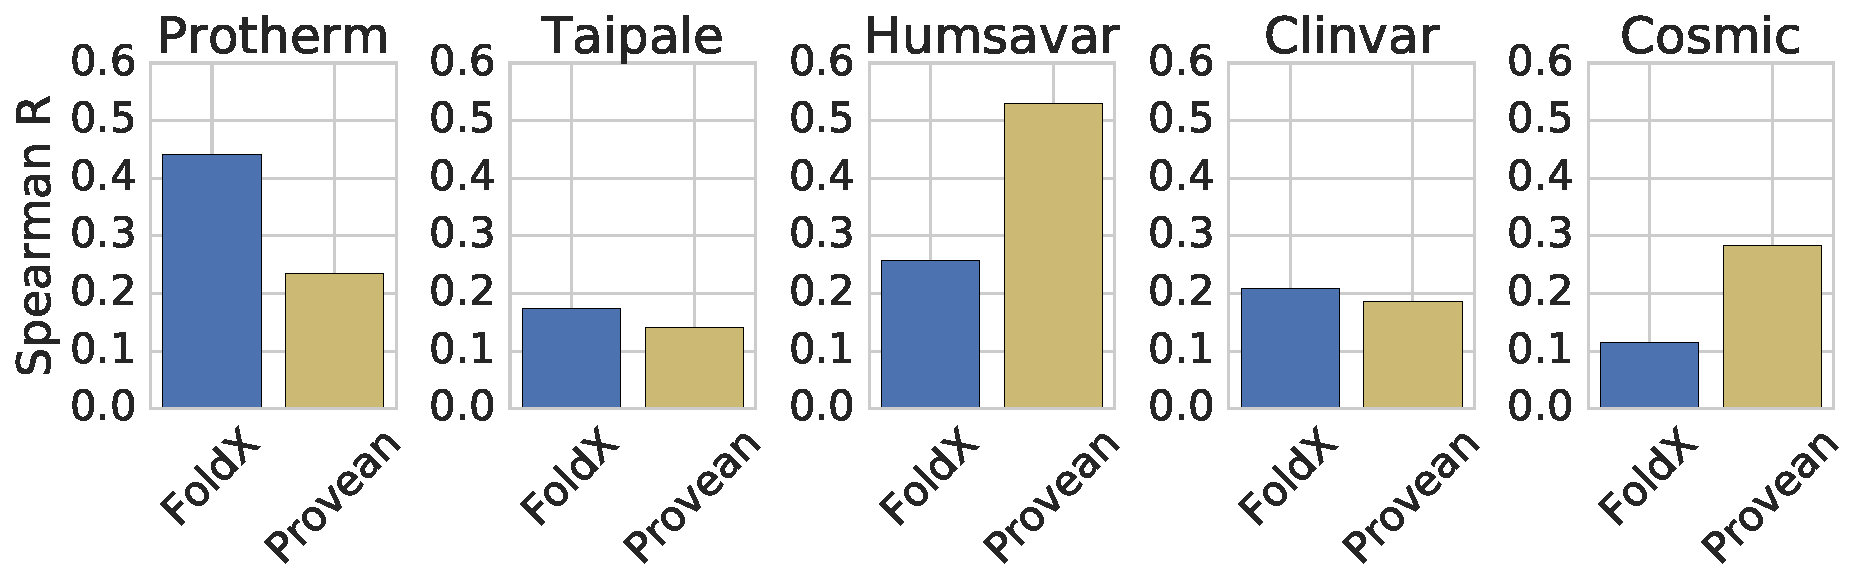
\includegraphics[width=1.0\linewidth]{static/elaspic_training_set/core_data_statistics/initial_performance.pdf}
	\caption{Performance on the training / validation datasets.}
\end{figure}

\begin{figure}[h]
	\centering
	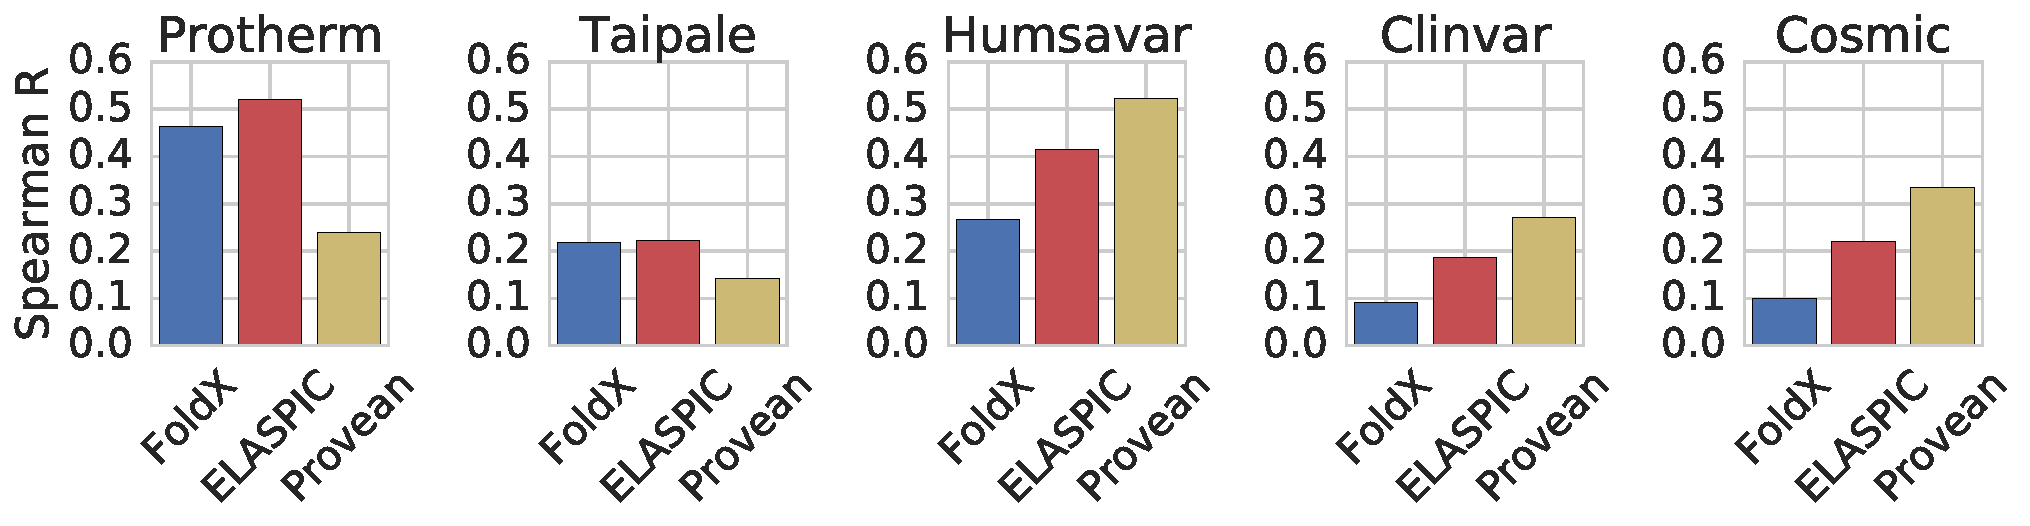
\includegraphics[width=1.0\textwidth]{static/elaspic_training_set/core_machine_learning/final_performance.pdf}
	\caption{Performance on the test datasets.}
\end{figure}

\clearpage

% Final results

\begin{table}[h]
\caption{Core features.} \label{tab:core_features}
\begin{tabular}{l | p{13cm}}
	\toprule
	Feature name & Feature description \\
	\midrule
	... & ... \\
	\bottomrule
\end{tabular}
\end{table}


\begin{table}[h]
\caption{Core parameters.} \label{tab:core_parameters}
\begin{tabular}{l | l | l}
	\toprule
	Parameter label & Parameter description & Parameter value \\
	\midrule
	... & ... \\
	\bottomrule
\end{tabular}
\end{table}


% === INTERFACE ===

% Training set stats

\begin{figure}[h]
	\centering
	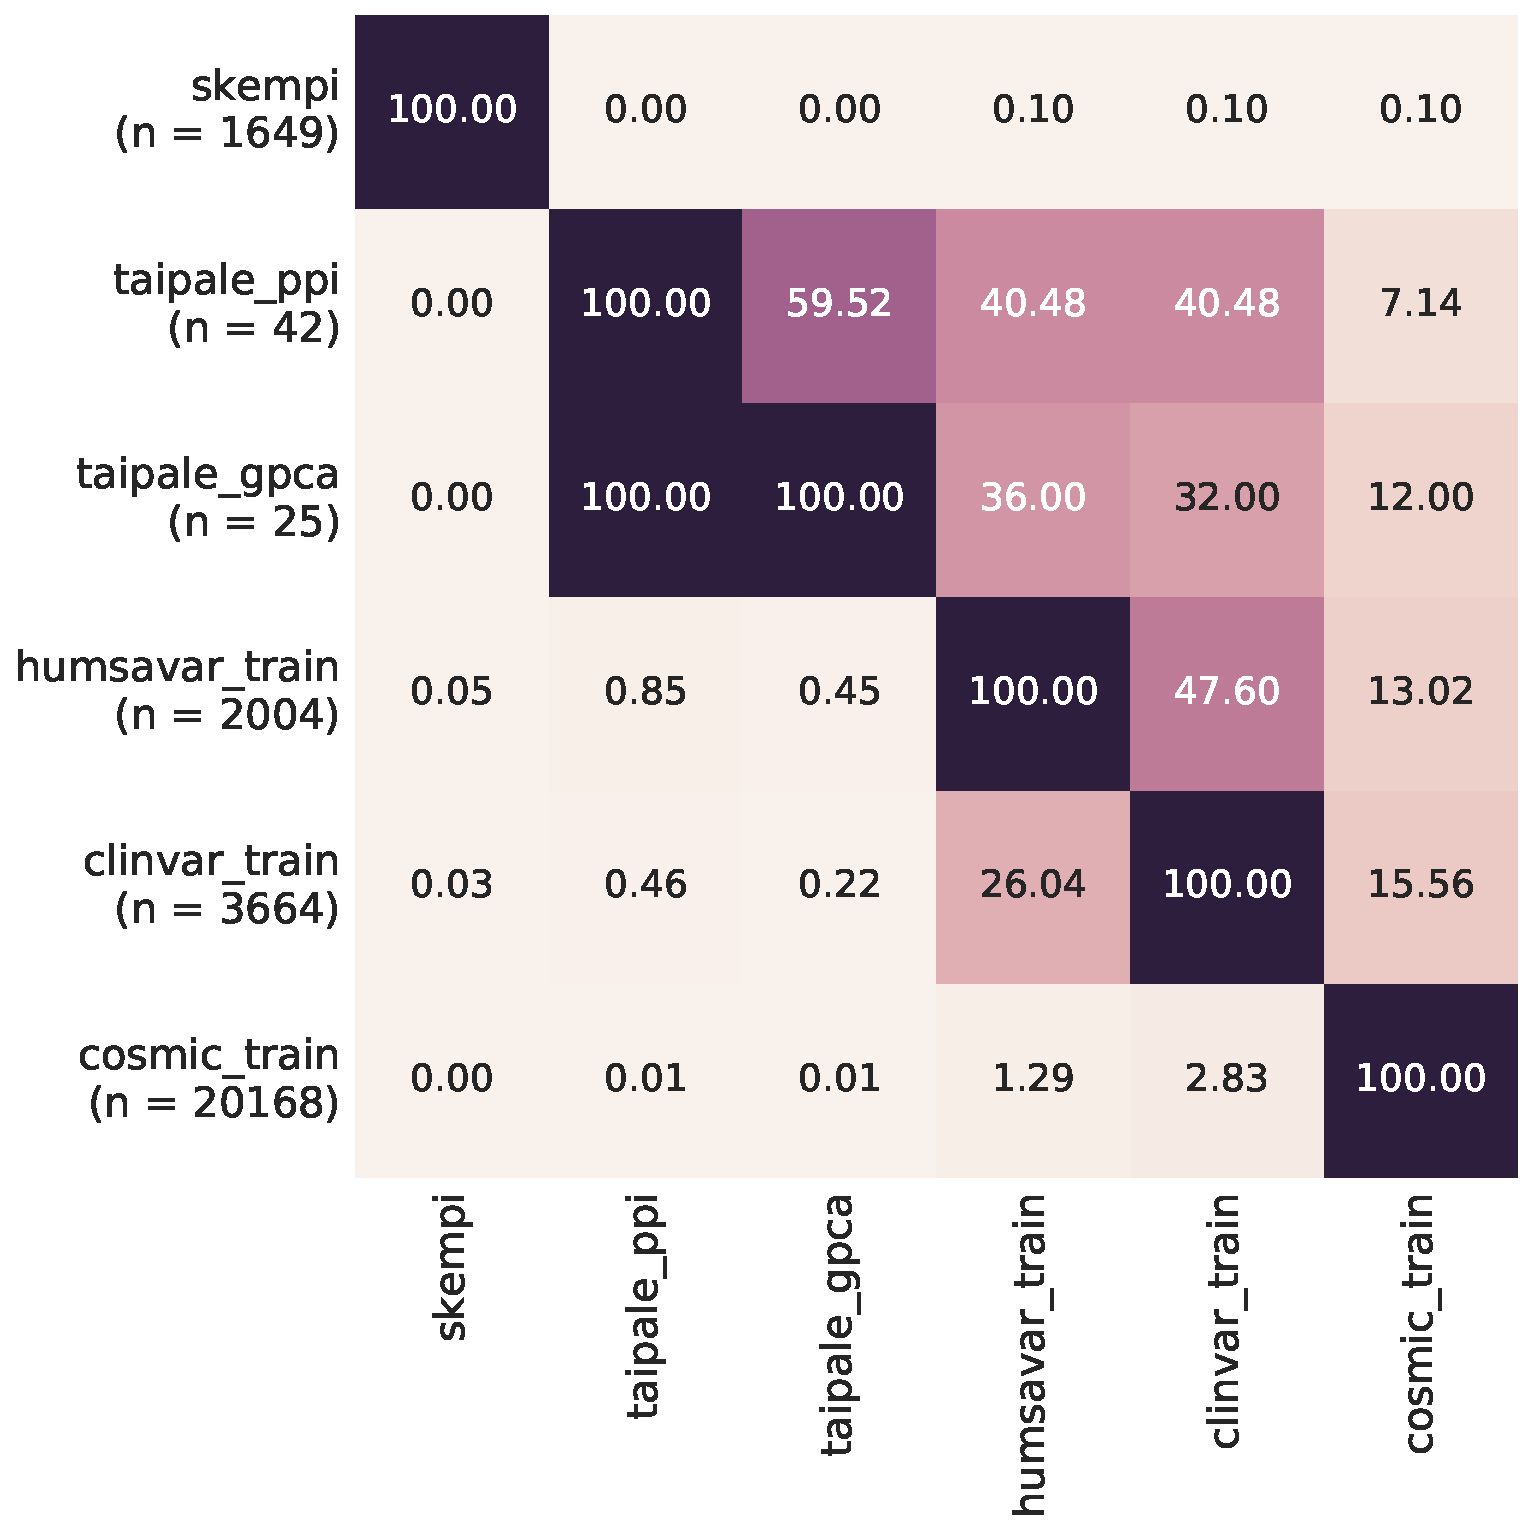
\includegraphics[width=0.65\textwidth]{static/elaspic_training_set/interface_data_statistics/training_set_overlap_final.pdf}
	\caption{Size and overlap between the core and interface predictor datasets.}
\end{figure}

\begin{table}[h]
\caption{Description of the dataset used to train the interface predictor.} \label{tab:interface_datasets}
\begin{tabular}{l | p{13cm}}
	\toprule
	Dataset name & Experimental feature \\
	\midrule
	Skempi \cite{kumar_protherm_2006} & Change in the Gibbs free energy of protein folding ($\Delta \Delta G$). \\
	Taipale \cite{sahni_widespread_2015} & Change in the interaction with various quality control factors (QCFs), measured using the LUMIER assay. \\
	Humsavar \cite{consortium_uniprot:_2015} & $1$ if the mutation is annotated with at least one disease in the UniProt \textit{humsavar.txt} file. $0$ if the mutation is annotated as ``Polymorphism'' in the UniProt \textit{humsavar.txt} file. \\
	ClinVar \cite{landrum_clinvar:_2016} & $1$ if the mutation is found in the ClinVar \textit{clinvar\_20160531.vcf} file. $0$ if the mutation is found in the ClinVar \textit{common\_no\_known\_medical\_impact\_20160531.vcf} file. \\
	COSMIC \cite{forbes_cosmic:_2015} & $1$ if the mutation is predicted to be deleterious by FATHMM in the COSMIC database. $0$ if the mutation is predicted to be benign by FATHMM in the COSMIC database. \\
	\bottomrule
\end{tabular}
\end{table}


% Machine learning

\begin{figure}[h]
	% \centering
	\begin{subfigure}[b]{0.6\textwidth}
		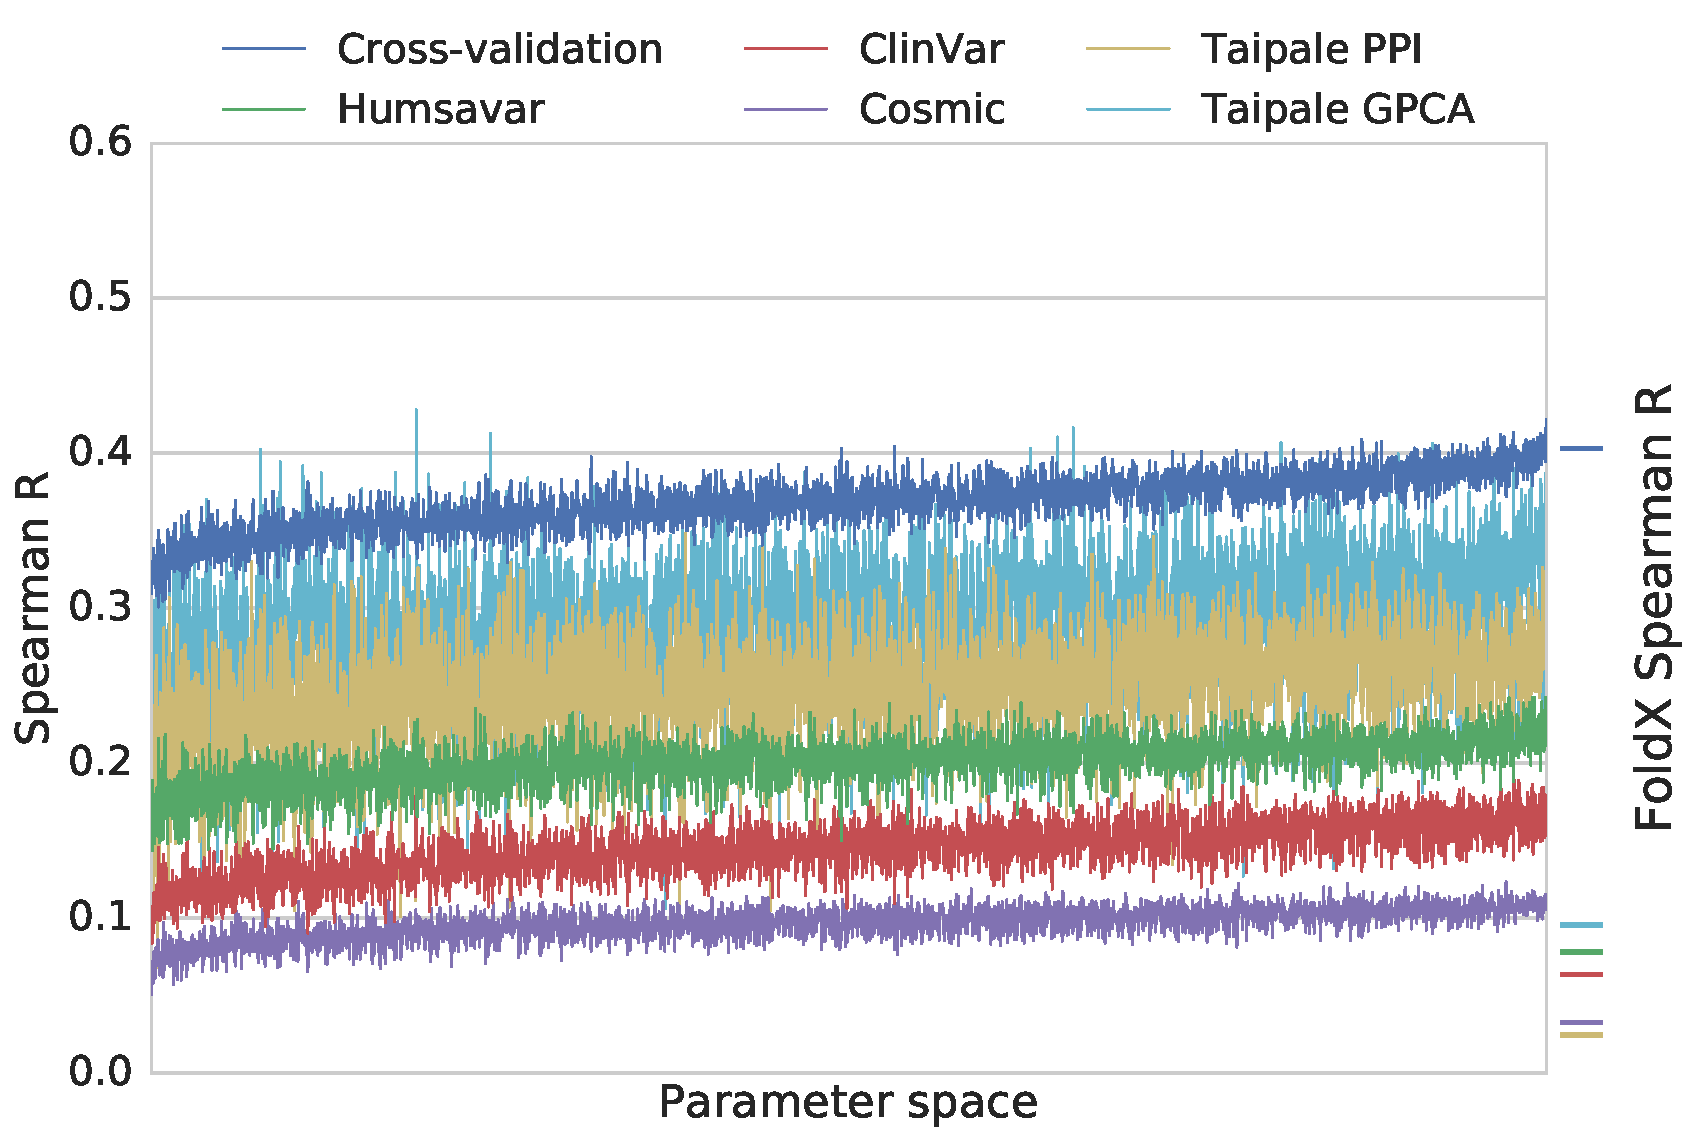
\includegraphics[width=1\linewidth]{static/elaspic_training_set/interface_machine_learning/gridsearch.pdf}
		\caption{Grid-search over parameter space.}
		\label{fig:Ng1}
	\end{subfigure}

	\begin{subfigure}[b]{0.75\textwidth}
		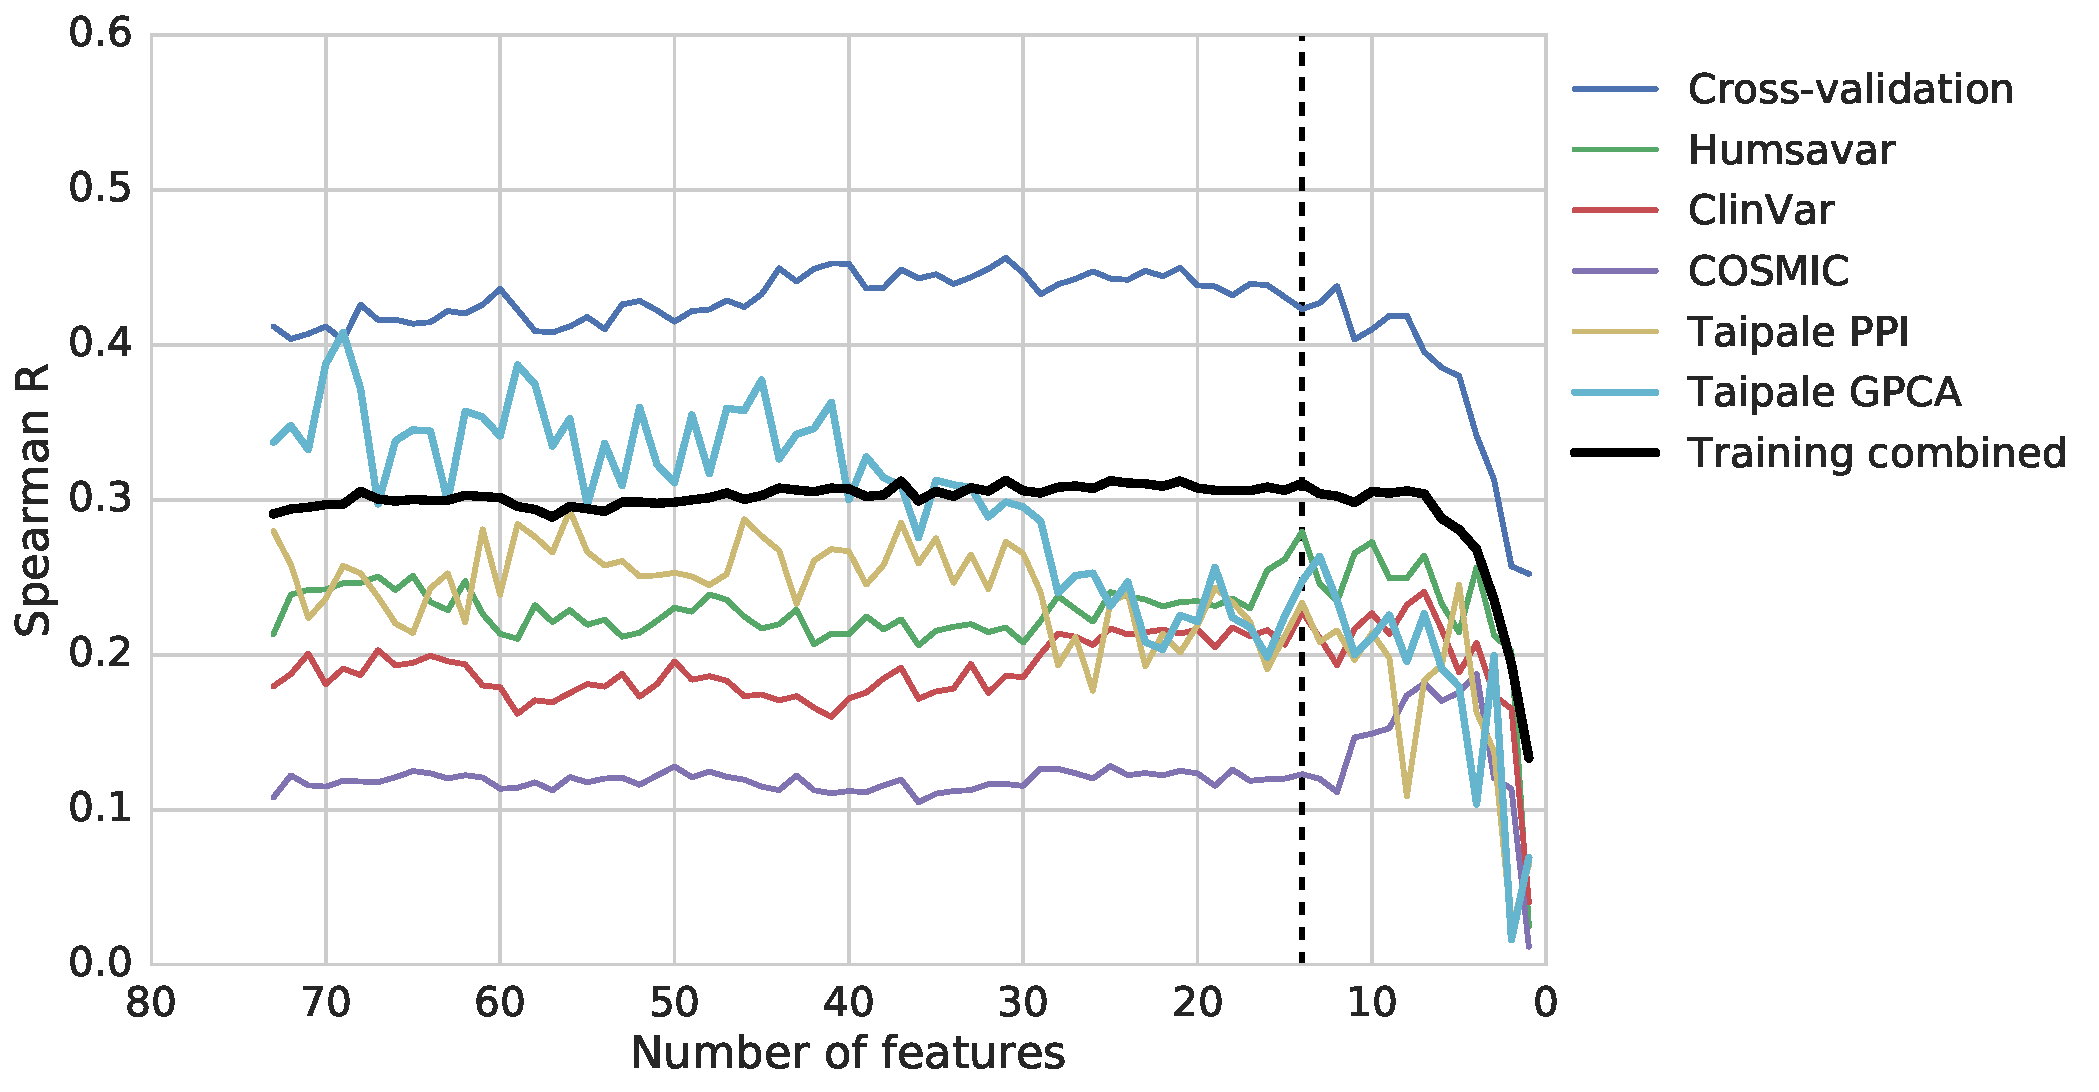
\includegraphics[width=1\linewidth]{static/elaspic_training_set/interface_machine_learning/feature_elimination.pdf}
		\caption{Feature elimination.}
		\label{fig:Ng1}
	\end{subfigure}

	\caption{Machine learning pipeline.}
\end{figure}



\begin{figure}[h]
	\centering
	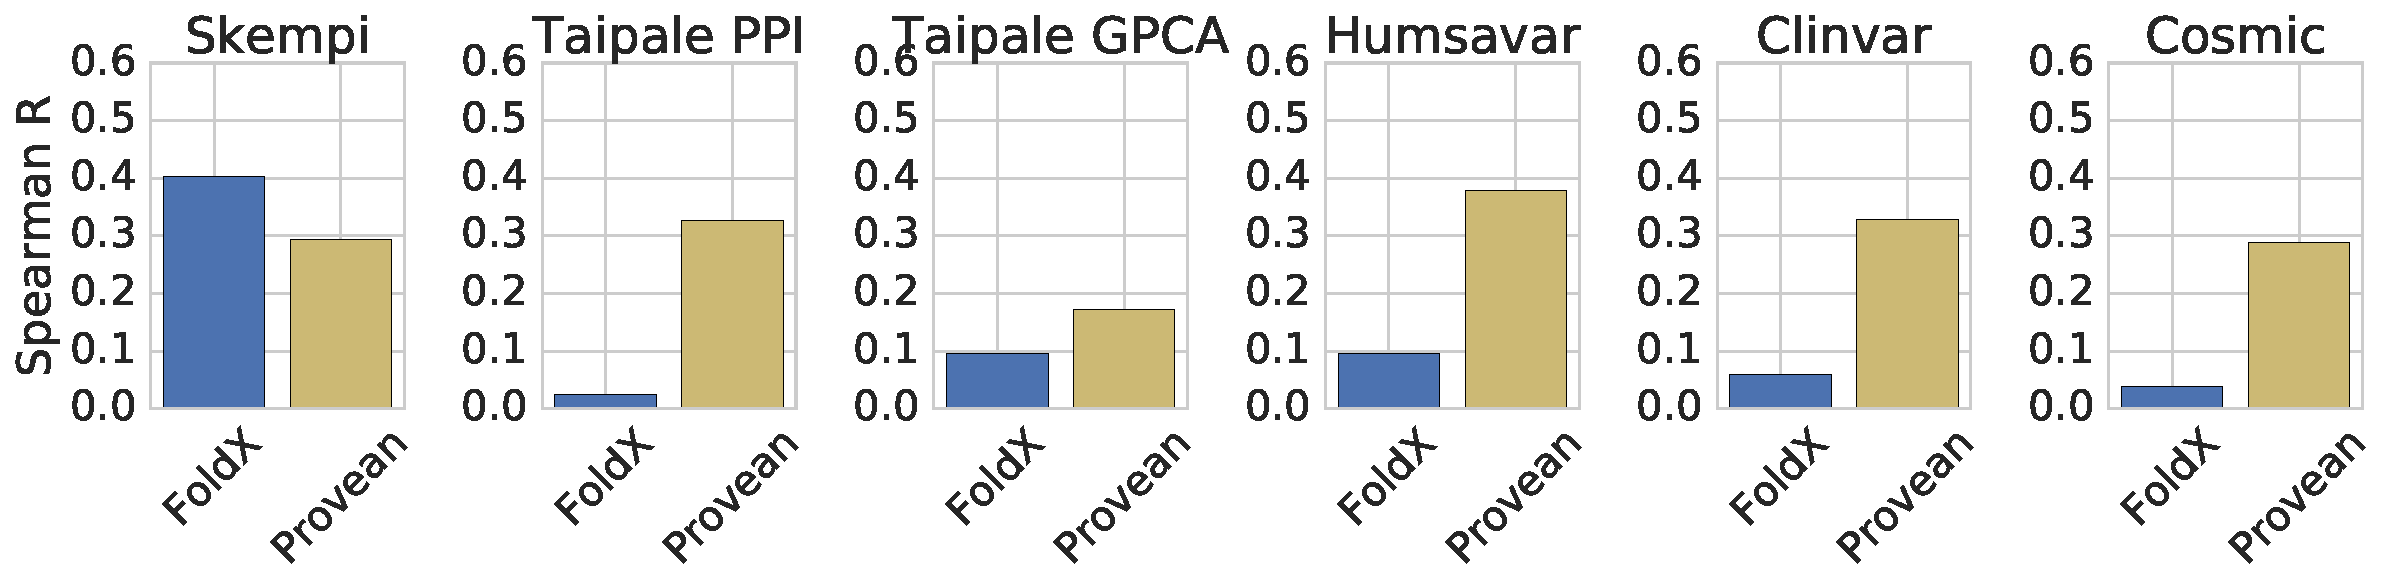
\includegraphics[width=1.0\linewidth]{static/elaspic_training_set/interface_data_statistics/initial_performance.pdf}
	\caption{Performance on the training / validation datasets.}.
\end{figure}

\begin{figure}[h]
	\centering
	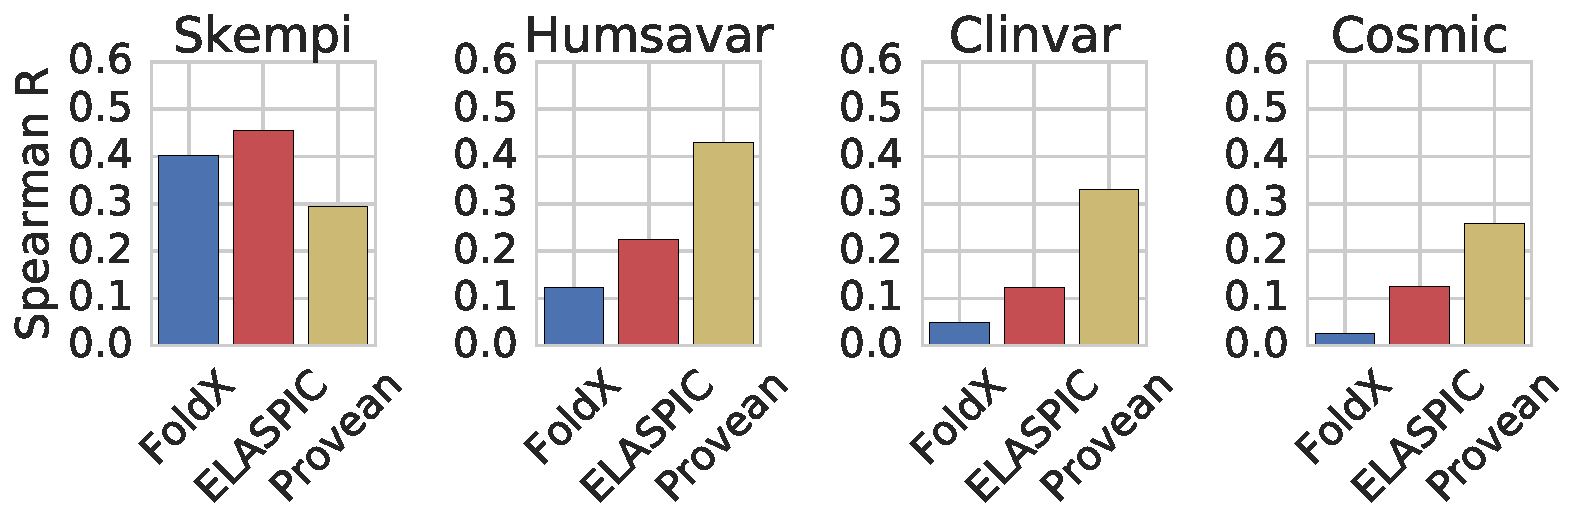
\includegraphics[width=1.0\textwidth]{static/elaspic_training_set/interface_machine_learning/final_performance.pdf}
	\caption{Performance on the test datasets.}
\end{figure}

\clearpage

% Final results

\begin{table}[h]
\caption{Interface features.} \label{tab:interface_features}
\begin{tabular}{l | p{13cm}}
	\toprule
	Feature name & Feature description \\
	\midrule
	... & ... \\
	\bottomrule
\end{tabular}
\end{table}


\begin{table}[h]
\caption{Interface parameters.} \label{tab:interface_parameters}
\begin{tabular}{l | l | l}
	\toprule
	Parameter label & Parameter description & Parameter value \\
	\midrule
	... & ... \\
	\bottomrule
\end{tabular}
\end{table}
